\chapter{Results}
\label{chap:results}
In this chapter we are going to present the obtained results using the previous models, both from a quantitative point of view, by measuring correlation coefficient over predicted data and from a qualitative point of view, by surveying a few listeners with predicted and real performance synthesis. Firstly, in Section~\ref{sec:ev_measures} we are going to explain what measures are we going to consider for both results analysis. In Section~\ref{sec:features} we are going to apply feature selection in order to see what features are more relevant in order to obtain better prediction for performance actions. In Section~\ref{sec:ev_results} we present separately the results from both evaluations, quantitative and qualitative. Finally, in Section~\ref{sec:discussion} we discuss the obtained results.

\section{Evaluation Measures}
\label{sec:ev_measures}
For the quantitative evaluation we are going to use Correlation Coefficient as evaluation metric. Correlation coefficient tells us how much predicted PAs and computed ones are related. It gives values between -1 and 1, where 0 is no relation, 1 is very strong linear relation and -1 is an inverse linear relation.

\section{Feature Selection}
\label{sec:features}

\begin{table}[ht!]
\centering
 
  \begin{tabular}{  l l p{6cm} }
    \hline
    Dataset & Best Subset & Ranked \\ \hline
    "All (onset\_dev)" & 6, 8, 9, 10, 13, 14, 17 &  6, 17, 8, 13, 10, 14, 9, 5, 27, 26, 24, 31, 20, 18, 16, 35, 23, 25, 32, 29, 12, 11, 22, 4, 19, 15, 33, 3, 7, 34, 21, 2, 30, 28, 1 \\
    "All (energy\_rat) & 6, 7, 9, 20, 21, 24, 27, 32 & 6, 7, 22, 32, 9, 24, 20, 27, 5, 35, 23, 31, 1, 8, 2, 10, 13, 14, 19, 4, 18, 26, 3, 17, 30, 11, 15, 33, 34, 25, 12, 28, 29, 21, 16  \\
    
    \hline
  \end{tabular}

 \caption[Selected Features using Ranker and Best Subset with wrapped Decision Tree]{Selected Features using Best Subset and Ranker with wrapped Decision Tree. Code for descriptors can be found in table~\ref{tab:note_descriptors}.}
  \label{tab:feature_selection}

\end{table}


In Table~\ref{tab:feature_selection} we present for each PA dataset, two different feature selection algorithms. In the middle column, best subset of features is shown and in the right column all features are ranked using Ranker with wrapped Decision Tree. As we can see, for \textit{Onset Deviation} we achieve the best performance with just 7 features out of 35, being those: \textit{Onset in seconds}, \textit{Measure}, \textit{Previous duration in beats}, \textit{Previous duration in seconds}, \textit{Previous inter-onset distance}, \textit{Next inter-onset distance} and \textit{Simultaneous notes}.

For \textit{Energy Ratio} we achieve the best performance with a subset of 8 features out of 35, being those: \textit{Onset in seconds}, \textit{Duration in seconds}, \textit{Previous duration in beats}, \textit{Key}, \textit{Note to key}, \textit{Chord type}, \textit{Metrical Strength} and \textit{Phrase}

In Figure~\ref{fig:feature_selection} we present the Correlation Coefficients (CC) between predicted and actual Performance Actions for Onset deviation and Energy Ratio while adding features by ranking order. In red we show the accuracy for the whole Train dataset and in blue the results with 10 fold Cross-Validation. For both PAs the best accuracy (using CV) was obtained with the set containing the first 5 best ranked features, as adding more features just makes CC decrease.



\begin{figure}[ht!]
\centering
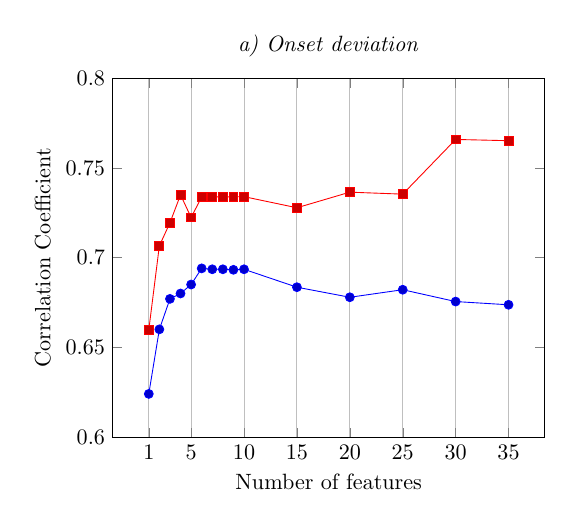
\begin{tikzpicture}[scale=0.8]

\begin{axis}[legend style={font=\scriptsize},
		title={\textit{a) Onset deviation}},
        ylabel={Correlation Coefficient},
        xlabel={Number of features},
        ymin=0.60,ymax=0.80,
        xtick={1,5,10,15,20,25,30,35},
        xmajorgrids]

    \addplot coordinates {(1,0.624) (2,0.660) (3,0.677) (4,0.680) (5,0.685) (6,0.694) (7, 0.6935)  (8, 0.6935) (9,0.6932) (10,0.6935) (15,0.6835) (20, 0.6779)  (25, 0.6821) (30, 0.6755) (35, 0.6737)};
    
    \addplot coordinates {(1, 0.6597) (2, 0.7066)  (3, 0.7194) (4, 0.735) (5, 0.7224) (6, 0.7338) (7, 0.7339) (8, 0.7339) (9, 0.7339) (10, 0.734) (15, 0.7278) (20, 0.7365) (25, 0.7354) (30, 0.7659) (35, 0.7652)};
     
  %  \addlegendentry{Onset\_dev cv10f}
   % \addlegendentry{Energy\_rat cv10f}

\end{axis}
\end{tikzpicture}
\qquad
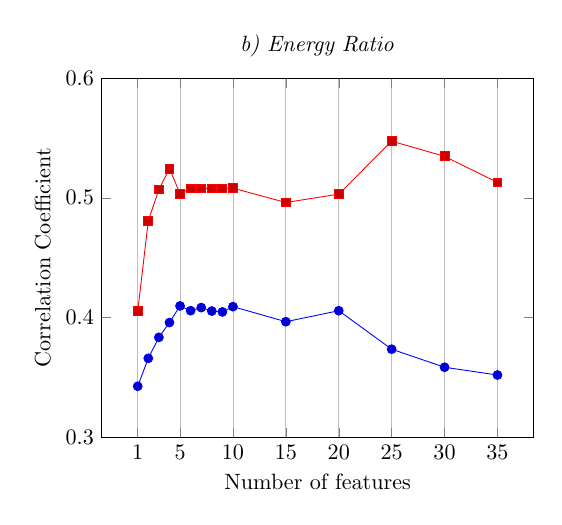
\begin{tikzpicture}[scale=0.8]

\begin{axis}[legend style={font=\scriptsize},
		title={\textit{b) Energy Ratio}},
        ylabel={Correlation Coefficient},
        xlabel={Number of features},
        ymin=0.30,ymax=0.60,
        xtick={1,5,10,15,20,25,30,35},
        xmajorgrids]

     \addplot coordinates { (1,0.3424) (2, 0.3658) (3, 0.3833) (4, 0.3957) (5, 0.4096) (6, 0.4056) (7, 0.4082) (8, 0.4053) (9, 0.4046) (10, 0.4090) (15, 0.3964) (20, 0.4056) (25, 0.3734) (30,0.3583) (35, 0.3518)};
     
     \addplot coordinates { (1, 0.4051) (2, 0.4808) (3, 0.507) (4, 0.5244) (5, 0.5035) (6, 0.5079) (7, 0.5079) (8, 0.5079) (9, 0.5079) (10, 0.5081) (15, 0.4961) (20, 0.5031) (25, 0.5474) (30, 0.5347) (35, 0.5129)};
    
  %  \addlegendentry{CrossValidation 10f}
   % \addlegendentry{Train dataset}

\end{axis}
\end{tikzpicture}

\caption[Results depending on the number of selected features.]{Results depending on the number of selected features according to table~\ref{tab:feature_selection}. Algorithm used: Decision Tree. Shown values correspond to Correlation Coefficients.}
\label{fig:feature_selection}
\end{figure}

\section{Evaluation Results}
\label{sec:ev_results}
In this section we present both quantitative and qualitative results. The proposed approach was quantitatively evaluated by measuring \textit{Correlation Coefficient} (CC) obtained with the models studied and qualitatively evaluated by asking listeners to compare predicted and real performances. 

\subsection{Quantitative evaluation}
In Table~\ref{tab:results_ml_cv} we show the results comparing different Machine Learning algorithms both with cross-validation and with the whole Train dataset. In the top half of the table we present the results by performance (1 \textit{Darn that dream} and 2 \textit{Suite en La}) and by Performance Action (\textit{Onset deviation} and \textit{Energy ratio}). In the bottom half of the table we merged those three performances into a big dataset and we present the results for this complete large ("All") dataset, for this large dataset with just the 5 top features ("$All_{5features}$", and for this large dataset with the best subset of features ("$All_{bestsubset}$").

Several machine learning algorithms have been tested for each one of this cases of study. From left to right: Decision Trees, K-Nearest Neighbours (K=1), K-Nearest Neighbours (K=2), K-Nearest Neighbours (k=4), Support Vector Machines and Artificial Neural Networks. All this models were computed using Weka.

\begin{table}
\centering
\caption[Results comparing different ML models (10 fold Cross-Validation)]{Results comparing different ML models (10 fold Cross-Validation). All datasets correspond to the three datasets merged into one. Shown values correspond to Correlation Coefficients.}
\label{tab:results_ml_cv}
\footnotesize
\begin{tabular} {lcccHcccH}
\\ \hline
\multirow{2}{3cm}{Dataset (feature)} & D.Tree & $k_1NN$ & $k_2NN$ & $k_4NN$ & $k_8NN$ & SVM & ANN & L.Reg \\ 
& cv/train & cv/train & cv/ train & cv/train & cv/train & cv/train & cv/train & cv/train\\\hline

'Darn (energy)' & 0.37/0.53 & 0.18/1 &  0.27/0.78 & 0.27/0.64 &  0.28/0.52 &  0.37/0.55 & 0.26/0.98 & 0.35/0.58 \\
'Darn (onset)' & 0.70/0.87 & 0.35/1 &  0.42/0.83 & 0.48/0.75 & 0.52/0.69 & 0.57/0.68 & 0.47/0.99 & 0.56/0.71  \\
'Suite (energy)' & 0.35/0.59 & 0.24/1 & 0.31/0.77 & 0.33/0.64 & 0.32/0.53 &  0.23/0.38 &  0.17/0.70 & 0.26/0.43 \\
'Suite (onset)' & 0.77/0.88 & 0.28/1 & 0.35/0.80 & 0.37/0.70 & 0.33/0.53 & 0.30/0.40 & 0.29/0.79 & 0.30/0.44 \\
'Suite2 (energy)' & 0.32/0.70 & 0.21/1 & 0.24/0.77 & 0.19/0.59 & 0.17/0.45 & 0.19/0.31 & 0.18/0.66 & 0.19/0.39 \\
'Suite2 (onset)' & 0.83/0.92 & 0.43/1 & 0.48/0.85 & 0.45/0.74 & 0.51/0.85 & 0.44/0.52 & 0.40/0.78 & 0.44/0.55 \\ \hline

'All (energy)' & 0.35/0.51 & 0.22/1 & 0.26/0.78 & 0.27/0.64 & 0.27/0.51 & 0.21/0.33 & 0.23/0.63 & 0.25/0.38 \\
'All (onset)' & 0.67/0.77 & 0.30/1 & 0.36/0.81 & 0.42/0.69 & 0.42/0.60 & 0.39/0.45 & 0.29/0.67 & 0.40/0.47 \\ 
'All (energy)'$_{5 features}$ & 0.41/0.50 & 0.30/1 & 0.37/0.80 & 0.39/0.67 & 0.37/0.57 & 0.14/0.21 & 0.14/0.36 & 0.16/0.23 \\
'All (onset)'$_{5 features}$ & 0.69/0.72 & 0.38/1 & 0.61/0.82 & 0.65/0.79 & 0.65/0.75 & 0.30/0.31 & 0.44/0.43 & 0.31/0.32 \\
'All (energy)'$_{best subset}$ & 0.41/0.51 & 0.30/1 & 0.37/0.79 & 0.38/0.66  & 0.37/0.57  & 0.16/0.21 & 0.15/039 & 0.15/0.23 \\
'All (onset)'$_{best subset}$ & 0.69/0.73 & 0.37/1 & 0.58/0.82 & 0.62/0.78 & 0.64/0.73 & 0.30/0.32 & 0.48/0.48 &  0.31\\

\hline
\end{tabular} 
\footnotesize

\end{table}



%\begin{table}
\centering
\caption[Results comparing different ML models (Train/Test)]{Results comparing different ML models (Train/Test). In this table 66\% of the Dataset has been used as Train and 33\% as Test. Notes has been randomly selected. Shown values correspond to Correlation Coefficients.}
\label{tab:results_ml_tt}
\footnotesize

\begin{tabular} {lcccccccc}
\\ \hline
Dataset (feature) & D.Tree& $k_1NN$ & $k_2NN$ & $k_4NN$ & $k_8NN$ & SVM & ANN & L.Reg \\ \hline
'Darn (energy\_rat)' & 0.44 & 0.14  & 0.21  & 0.23  & 0.31  & 0.32  & 0.34  & 0.35 \\
'Darn (onset\_dev)' & 0.58 & 0.41  & 0.49  & 0.44  & 0.41  & 0.56  & 0.39  & 0.51 \\
'Suite (energy\_rat)' & 0.33 & 0.30  & 0.27  & 0.27  & 0.31  & 0.19  & 0.21  & 0.23 \\
'Suite (onset\_dev)' & 0.67 & 0.32  & 0.43  & 0.44  & 0.42  & 0.35  & 0.39  & 0.39 \\
'Suite2 (energy\_rat)' & 0.31 & 0.21  & 0.17  & 0.15  & 0.06  & 0.11  & 0.23  & 0.12 \\
'Suite2 (onset\_dev)' & 0.79 & 0.37  & 0.51  & 0.48  & 0.56  & 0.45  & 0.44  & 0.49 \\

\hline
\end{tabular}


\footnotesize

\end{table}

In Table~\ref{tab:results_mixed} we show the results of training with one dataset and testing with another one. This results are generated using Decision Trees and Artificial Neural Networks as they show to be the best algorithms in Table~\ref{tab:results_ml_cv}. As we can see, the results are very poor as we are mixing two very different music styles (a Jazz standard and a Classical piece). We also can see that if we train and test with different performances of the same score we achieve a Correlation Coefficient around 0.3 which might indicate that PAs are more performance dependant than piece dependant.
\begin{table}
\centering

\footnotesize
\begin{tabular} {llccHHcc}
\\ \hline

%% & \multicolumn{2}{c}{$k_1NN$}

 \multirow{2}{1cm}{Train} &  \multirow{2}{1cm}{Test} & \multicolumn{2}{c}{D.Tree} & & & \multicolumn{2}{c}{ANN}\\ 
 &  & energy & onset & energy & onset & energy & onset	 \\ \hline
'Darn' & 'Suite' & 0.013 & 0.156 & 0.110 & 0.069 & 0.047 & 0.008 \\
'Darn' & 'Suite2' & 0.091 & 0.183 & 0.018 & 0.177 & 0.033 & 0.075 \\
'Suite' & 'Darn' & 0.017 & 0.140 & 0.333  & 0.11 & 0.107 & 0.032 \\
'Suite' & 'Suite2' &  0.324 & 0.392 & 0.215 & 0.338 & 0.148 & 0.253 \\
'Suite2' & 'Darn' & 0.043 & 0.099 & 0.061 & 0.1672 & 0.079 & 0.027 \\
'Suite2' & 'Suite' & 0.240 &  0.384 & 0.2316 & 0.349 & 0.190 & 0.227 \\
\hline
\end{tabular} 
\footnotesize

\caption[Results mixing songs for Train/Test]{Results mixing songs for Train/Test. Whole song Datasets have been used in order to train or test. Shown values correspond to Correlation Coefficients.}
\label{tab:results_mixed}

\end{table}


\subsection{Qualitative evaluation}

For the qualitative survey, several synthesised pieces obtained by the models were compared to both the score (dead pan synthesis) and the performed (synthesised version) piece. Participants were asked to to guess how "human" they sounded by comparing among them through an on-line survey. Please see Appendix~\ref{app:survey} for a complete overview of the On-line survey.
They were given 4 different tests with three excerpts each one (Performance, Prediction and Score synthesis) and were asked to rate from 0 to 100 the "humanness" of each one related to the other two.

In Table~\ref{tab:survey_results_redux} we can see the median and average punctuation (over 12 participants) that each concrete audio was given. As we can see, the on-line survey consisted on 4 different excerpts with three different synthesis each one (a Performance synthesis, a Predicted synthesis and a plain Score synthesis). As we saw on the previous Figure~\ref{fig:survey} values for Performance and Prediction are very close and there is a little preference for Score synthesised midis.

\begin{table}
\centering
 
  \footnotesize
\begin{tabular}{l|ccc|ccc|ccc|ccc}

\hline
& \multicolumn{3}{c|}{intro1} & \multicolumn{3}{c|}{intro2} & \multicolumn{3}{c|}{middle}  & \multicolumn{3}{c}{end} \\ 
& Perf & Pred & Score & Perf & Pred & Score & Perf & Pred & Score & Perf & Pred & Score \\ \hline

Med & 40 & 39 & 50	& 63 & 46 & 76 & 45 & 52 & 68 & 42 & 42 & 69 \\
Avg & 41 & 43 & 52 & 59 & 48 & 71 & 47 & 48 & 65 & 44 & 46 & 69\\ \hline
\end{tabular}


 \caption[Numeric results of the on-line survey.]{Numeric results of the on-line survey.}
  \label{tab:survey_results_redux}
\end{table}
\begin{figure}[!ht]
\centering
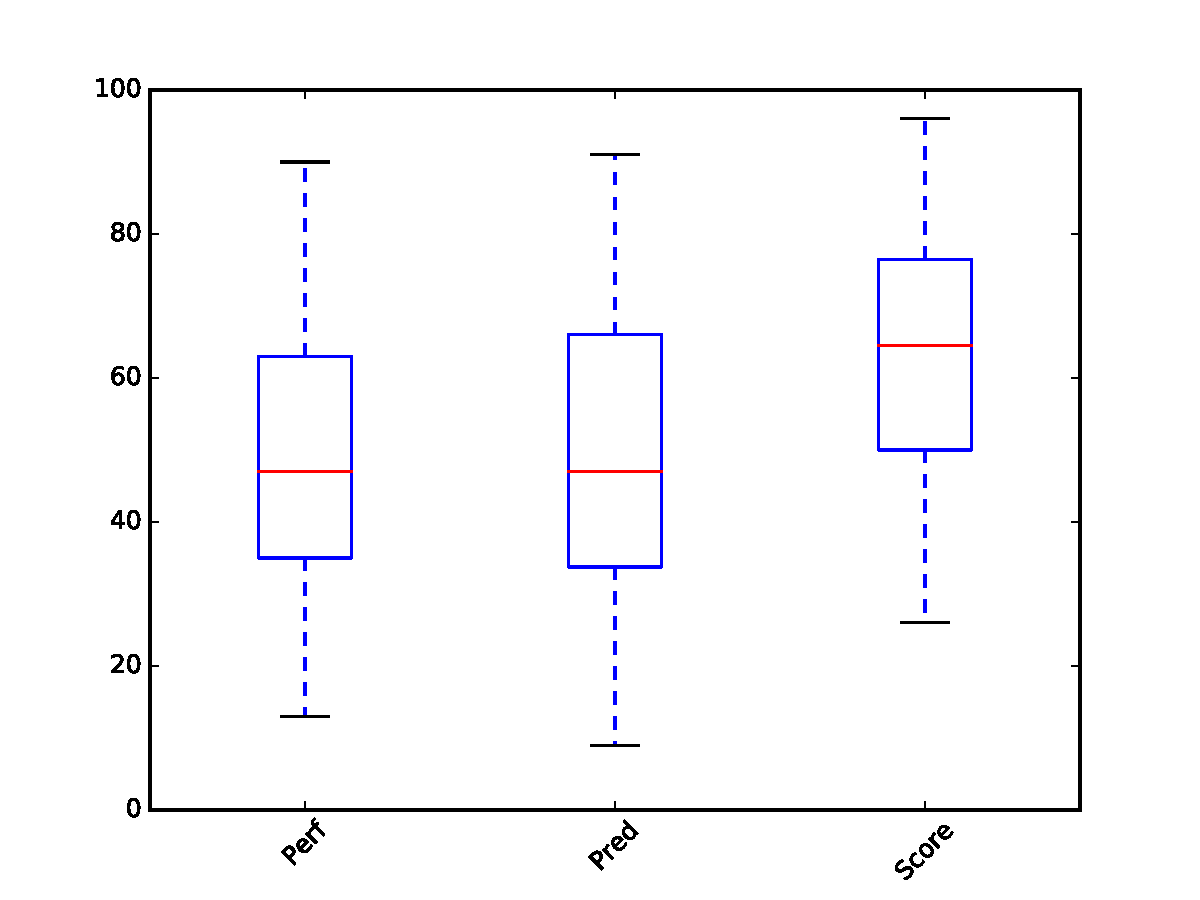
\includegraphics[width=0.7\textwidth]{Figures/survey.pdf}
\caption{Results of the on-line survey with performance, predicted and score synthesised midis.}
\label{fig:survey}
\end{figure}


In Figure~\ref{fig:survey} we display all On-line survey results gathered by type. I shows that participants perceived the score synthesis more "human" than the actual performance and predicted score. However, we obtained similar results among the performed piece and the predicted one, which might indicate that our models predictions are close to actual human performances. Full survey results can be found at Appendix~\ref{app:survey}.



\section{Discussion}
\label{sec:discussion}
Analysing the information provided in previous sections it can be seen that: in general, the algorithm which achieves better results using 10 fold Cross-validation is the Decision Trees, outperforming the three proposed K-NN, Support vector machines and artificial neural networks.

Figures~\ref{fig:onset} and \ref{fig:energy} show an excerpt of \textit{Onset deviation} and \textit{Energy ratio} predictions obtained with Decision Trees, respectively. The curves show \textit{Onset deviation} with respect the score, and \textit{Energy ratio} with respect to the mean loudness . The blue lines correspond to the deviations performed by the musician in the performance, and the red lines correspond to the deviation predicted by the model. In both figures it is shown how the model follows in a consistent way the deviations done in time and energy by the performer.

\begin{figure}
\centering
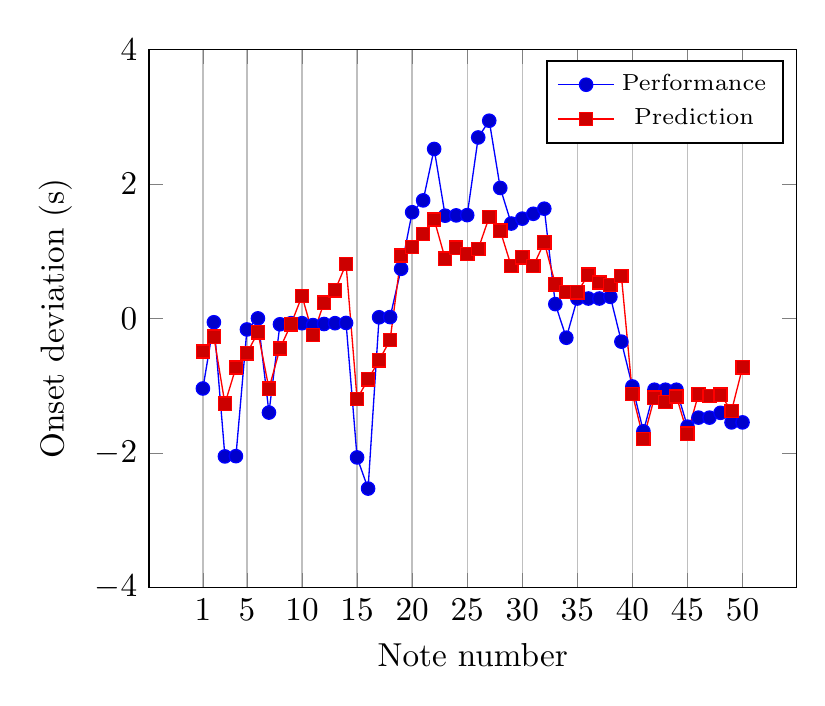
\begin{tikzpicture}[scale=1.2]

\begin{axis}[legend style={font=\scriptsize},
		ylabel={Onset deviation (s)},
        xlabel={Note number},
        ymin=-4, ymax=4,
        xtick={1,5,10,15,20,25,30,35,40,45,50},
        xmajorgrids]

    \addplot coordinates {(1,-1.042) (2,-0.057) (3,-2.052) (4,-2.048) (5,-0.164) (6,0.001) (7,-1.4) (8,-0.087) (9,-0.071) (10,-0.071) (11,-0.099) (12,-0.083) (13,-0.071) (14,-0.067) (15,-2.067) (16,-2.53) (17,0.017) (18,0.02) (19,0.738) (20,1.579) (21,1.755) (22,2.52) (23,1.528) (24,1.532) (25,1.536) (26,2.691) (27,2.94) (28,1.94) (29,1.411) (30,1.484) (31,1.556) (32,1.632) (33,0.213) (34,-0.287) (35,0.296) (36,0.296) (37,0.296) (38,0.321) (39,-0.345) (40,-1.012) (41,-1.679) (42,-1.06) (43,-1.06) (44,-1.06) (45,-1.609) (46,-1.475) (47,-1.475) (48,-1.404) (49,-1.546) (50,-1.546)};
    
     \addlegendentry{Performance}
    
    \addplot coordinates {(1,-0.492) (2,-0.273) (3,-1.267) (4,-0.73) (5,-0.519) (6,-0.206) (7,-1.043) (8,-0.447) (9,-0.087) (10,0.334) (11,-0.245) (12,0.233) (13,0.418) (14,0.809) (15,-1.197) (16,-0.906) (17,-0.624) (18,-0.321) (19,0.936) (20,1.06) (21,1.256) (22,1.471) (23,0.889) (24,1.054) (25,0.957) (26,1.032) (27,1.508) (28,1.304) (29,0.778) (30,0.91) (31,0.778) (32,1.132) (33,0.508) (34,0.393) (35,0.388) (36,0.652) (37,0.534) (38,0.496) (39,0.633) (40,-1.123) (41,-1.791) (42,-1.177) (43,-1.242) (44,-1.161) (45,-1.712) (46,-1.129) (47,-1.151) (48,-1.135) (49,-1.374) (50,-0.728)};
  
   \addlegendentry{Prediction}

\end{axis}
\end{tikzpicture}

\caption[Onset deviation in performance and prediction]{Onset deviation in performance and prediction}
\label{fig:onset}
\end{figure}
\begin{figure}
\centering
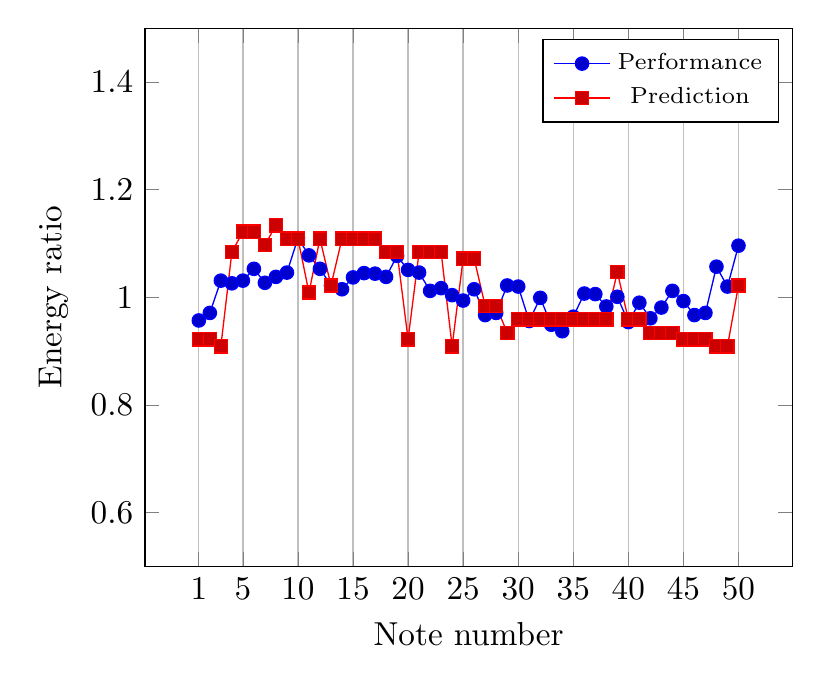
\begin{tikzpicture}[scale=1.2]

\begin{axis}[legend style={font=\scriptsize},
		ylabel={Energy ratio},
        xlabel={Note number},
        ymin=0.5, ymax=1.5,
        xtick={1,5,10,15,20,25,30,35,40,45,50},
        xmajorgrids]

    \addplot coordinates {(1,0.957) (2,0.971) (3,1.031) (4,1.026) (5,1.031) (6,1.053) (7,1.027) (8,1.038) (9,1.046) (10,1.11) (11,1.078) (12,1.053) (13,1.022) (14,1.015) (15,1.037) (16,1.045) (17,1.044) (18,1.038) (19,1.077) (20,1.051) (21,1.046) (22,1.012) (23,1.017) (24,1.004) (25,0.994) (26,1.015) (27,0.967) (28,0.971) (29,1.022) (30,1.02) (31,0.956) (32,0.999) (33,0.949) (34,0.937) (35,0.964) (36,1.007) (37,1.006) (38,0.983) (39,1.001) (40,0.954) (41,0.99) (42,0.961) (43,0.981) (44,1.012) (45,0.993) (46,0.967) (47,0.971) (48,1.057) (49,1.02) (50,1.096)};
  

    \addplot coordinates {(1,0.922) (2,0.922) (3,0.909) (4,1.084) (5,1.122) (6,1.122) (7,1.097) (8,1.134) (9,1.109) (10,1.109) (11,1.009) (12,1.109) (13,1.022) (14,1.109) (15,1.109) (16,1.109) (17,1.109) (18,1.084) (19,1.084) (20,0.922) (21,1.084) (22,1.084) (23,1.084) (24,0.909) (25,1.072) (26,1.072) (27,0.984) (28,0.984) (29,0.934) (30,0.959) (31,0.959) (32,0.959) (33,0.959) (34,0.959) (35,0.959) (36,0.959) (37,0.959) (38,0.959) (39,1.047) (40,0.959) (41,0.959) (42,0.934) (43,0.934) (44,0.934) (45,0.922) (46,0.922) (47,0.922) (48,0.909) (49,0.909) (50,1.022)};
    
     \addlegendentry{Performance}
    

   \addlegendentry{Prediction}

\end{axis}
\end{tikzpicture}

\caption[Energy Ratio in performance and prediction]{Energy Ratio in performance and prediction}
\label{fig:energy}
\end{figure}

In Figure~\ref{fig:predicted_darn} we can see a piano-roll representation of the first 20 notes with predicted Onsets. As we can see the model follows the typical strumming guitar pattern by playing first the low strings and then the higher ones. This strumming pattern was visible in the performance transcription (see Figure~\ref{fig:darn_20n}) where notes were played (\textit{arpeggiated}) from low pitch to high pitch so we can also visually see that our models represent the performance actions done by the player.

\begin{figure}[!ht]
\centering
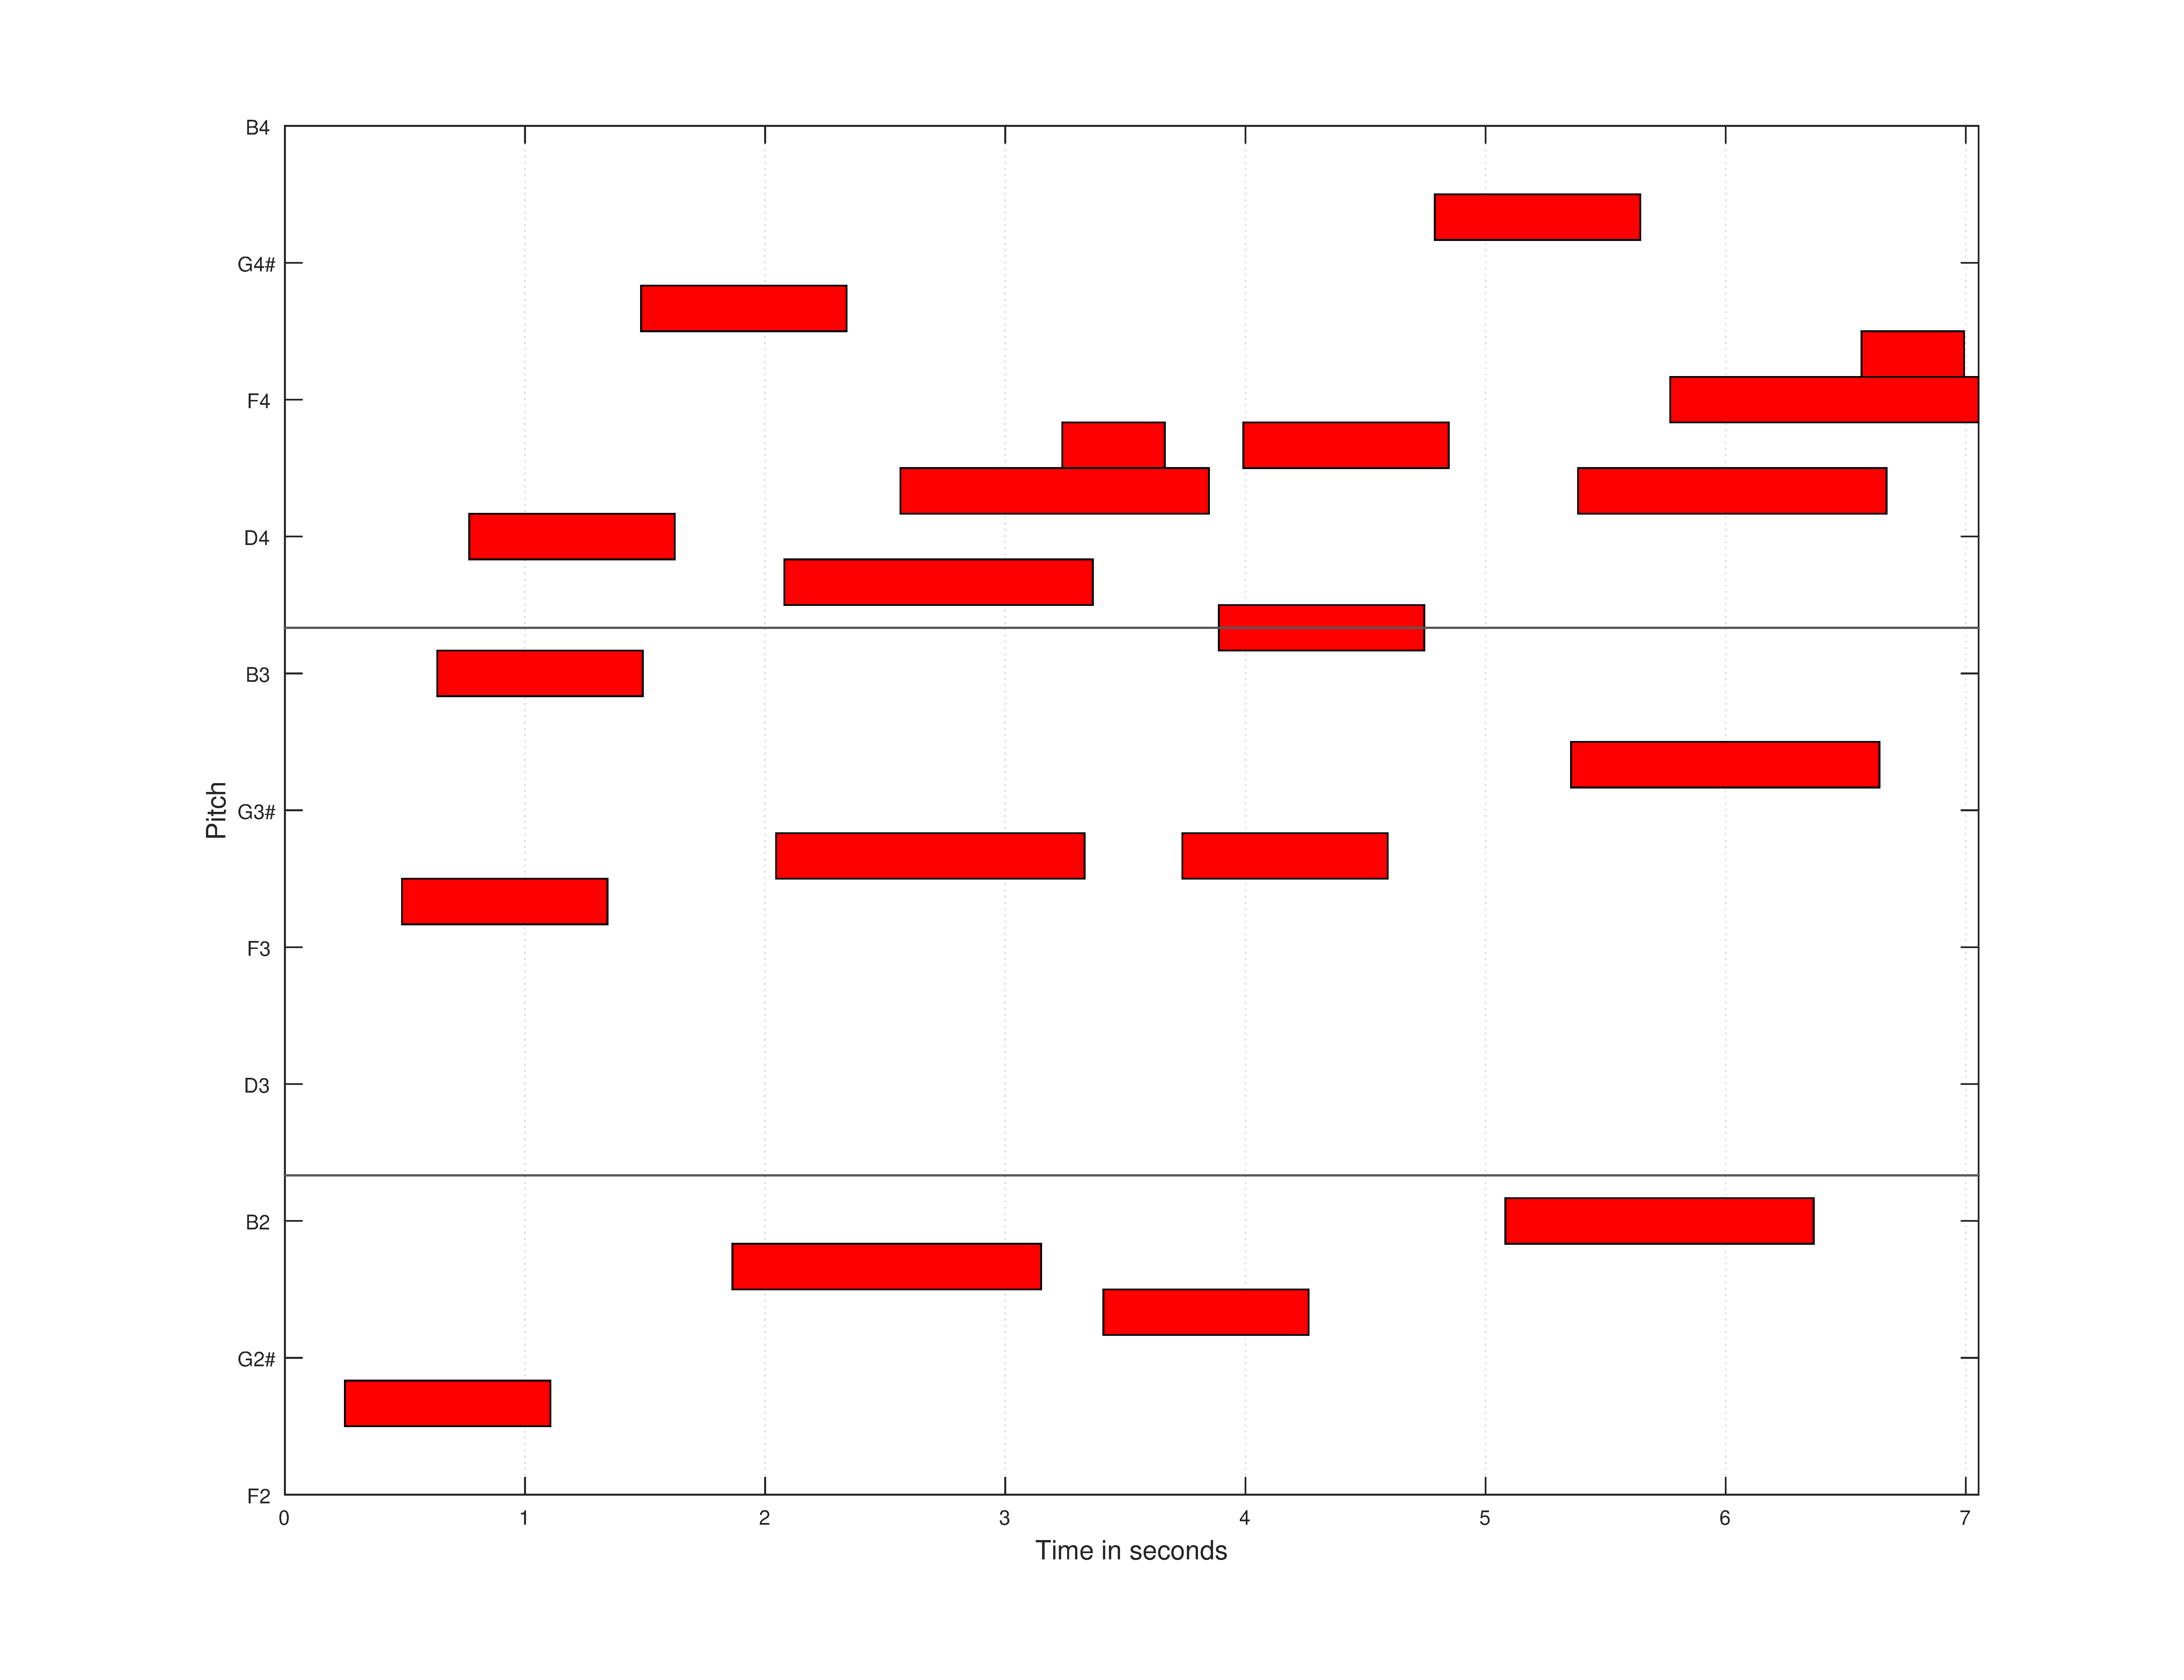
\includegraphics[width=0.8\textwidth]{Figures/Darn_all_predicted.pdf}
\caption{\textit{Darn that dream} first 20 notes predicted with piano-roll representation.}
\label{fig:predicted_darn}
\end{figure}


In Figure~\ref{fig:comparison} we can see how feature selection helps us to improve the results obtained. In the Y-axis we plot the Correlation Coefficient while bars represent different datasets by using all features, the best subset or the 5 best ranked features. Displayed values are obtained from the bottom half of Table~\ref{tab:results_ml_cv}. We can see that by using best subset (red column) or 5 best ranked features (green column) we can improve the Correlation Coefficient by the same amount as we obtain the same results with both feature selection algorithms.
\begin{figure}[ht!]
\centering
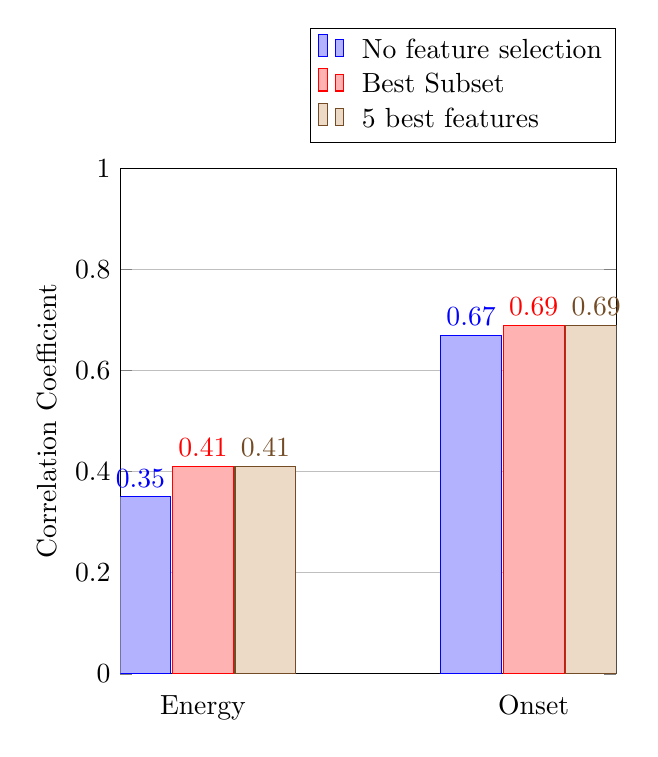
\begin{tikzpicture}
    \begin{axis}[
    	nodes near coords,
        width  = 0.65*\textwidth,
        height = 8cm,
        major x tick style = transparent,
        ybar=0.6,
        bar width=22pt,
        ymajorgrids = true,
        enlarge x limits = 0.5,
        ylabel = {Correlation Coefficient},
        symbolic x coords={Energy, Onset},
        xtick = data,
        scaled y ticks = false,
        enlarge x limits=0.25,
        ymin=0, ymax=1,
        legend cell align=left,
        legend style={
                at={(1,1.05)},
                anchor=south east,
                column sep=1ex
        }
    ]
        \addplot
            coordinates {(Energy, 0.35) (Onset,0.67)};

        \addplot
            coordinates {(Energy, 0.41) (Onset,0.69)};

        \addplot
            coordinates {(Energy, 0.41) (Onset,0.69)};


        \legend{No feature selection,Best Subset, 5 best features}
    \end{axis}
\end{tikzpicture}
\caption[Results with feature selection comparison.]{Results with feature selection comparison using Decision Trees. In this plot we use the "All" dataset.}
\label{fig:comparison}
\end{figure}

This results are very important as they show that with just a few features (~5 features) we can obtain better results than with all features (35 features), so probably it makes no sense to research on adding more and more features to the system but to improve those that obtained a better ranking using feature selection.

Our assumption about why the score synthesis is graded better than the performance or the prediction in the qualitative evaluation is that the virtual instrument does not synthesise very well the guitar and when two notes are played with very short inter-onset time it creates very strange artefacts. Moreover, as it is a midi synthesis we are used to hear it very perfect as it always comes from a music score, so introducing those artefacts and time deviations can sound really strange to us, as if the score wasn't well written.

One of the comments received in the On-line survey was: 
\begin{quote}
\textit{I based my "humanness" mainly in the attack of the instrument, when the time between one attack and the next is really short, it feels robotic and hasty. I tried not to guide myself on synthesis but it is difficult. The best of my grades went to a somehow "slower" performance with more "rallentando" than the other versions.} 
\end{quote}

This comment reinforces our assumption that the problem of higher punctuation to the score synthesis is due to the MIDI synthesis and the artefacts added when two onsets are really close. As the user says, it is very difficult to rate "humanness" from a MIDI synthesis as the sound itself is not human. 

Another comment on the survey reflects the difficulty of rating "humanness".  The "human" term could be some how ambiguous as it may refer to the smoothness of the performance or to the compositional aspect. In general we found that the qualitative evaluation is subjected to different perceptual aspects (mainly to the guitar synthesis) that are out of the main focus of this thesis work.  However, from this qualitative evaluation we can state two things: firstly, this is not a valid experiment to rate how "human" the predictions are as the users prefer score synthesis over synthesised human performances. Secondly, we think that this evaluation is a valid experiment in order to confirm that our predictions and models are really close to actual human performances. 



\cleardoublepage

